\newpage
\begin{center}
\noindent\textbf{ГЛАВА 3. ВЕРХНИЕ ОЦЕНКИ ХРОМАТИЧЕСКИХ ЧИСЕЛ СФЕР}\label{chapters:3}
\vspace{1.5mm}
\end{center}

\vspace{5pt}
\textbf{3.1 Численные эксперименты}\label{chapters:3.1}
\vspace{5pt}

sdfg asd f


asdf as df


asdf asd f


asdf as df

\begin{table}[h]
\centering
\captionsetup{justification=centering}
\caption{Сравнение эффективности \textit{SAT}-решателей при раскраске графа в $10$ цветов для различных $N$.} 
\label{chapter3:tab:color10}
\begin{tabular}{@{}|c|c|c|c|c|c|c|c|} 
\Xhline{4\arrayrulewidth}
SAT-решатель          & $192$ & $195$ & $212$ & $282$ & $358$ & $372$ & $400$ \\ \Xhline{4\arrayrulewidth}
lingeling             & 0.197 & 0.161 & 0.196 & 0.194 & 0.238 & 0.26  & 0.266 \\ \hline
Glucose               & 0.054 & 0.054 & 0.055 & 0.075 & 0.095 & 0.095 & 0.105 \\ \hline
MiniSat               & 0.054 & 0.054 & 0.054 & 0.074 & 0.09  & 0.091 & 0.105 \\ \hline
CryptoMiniSat         & 0.025 & 0.024 & 0.026 & 0.034 & 0.035 & 0.037 & 0.039 \\ \hline
Cadical               & 0.032 & 0.034 & 0.037 & 0.038 & 0.035 & 0.042 & 0.051 \\ \hline
MapleCOMSPS-CHB       & 0.061 & 0.044 & 0.049 & 0.071 & 0.075 & 0.08  & 0.097 \\ \hline
MapleCOMSPS-LRB       & 0.053 & 0.044 & 0.045 & 0.066 & 0.075 & 0.077 & 0.083 \\ \Xhline{4\arrayrulewidth}
\end{tabular}
\end{table}

asdfdsaf
asdf
sdaf

\begin{table}[h]
\centering
\captionsetup{justification=centering}
\caption{Сравнение эффективности \textit{SAT}-решателей при раскраске графа в $9$ цветов для различных $N$.}
\label{chapter3:tab:color9}
\begin{tabular}{@{}|c|c|c|c|c|c|c|c|}
\Xhline{4\arrayrulewidth}
SAT-решатель          & $192$ & $195$ & $212$ & $282$ & $358$ & $372$ & $400$ \\ \Xhline{4\arrayrulewidth}
lingeling             & 0.237 & 0.262 & 0.338 & 0.35  & 0.385 & 0.258 & 0.287 \\ \hline
Glucose               & 0.088 & 0.075 & 0.064 & 0.056 & 0.094 & 0.136 & 0.207 \\ \hline
MiniSat               & 0.088 & 0.054 & 0.058 & 0.124 & 0.068 & 0.096 & 0.117 \\ \hline
CryptoMiniSat         & 0.059 & 0.024 & 0.024 & 0.137 & 0.054 & 0.272 & 0.063 \\ \hline
Cadical               & 0.095 & 0.034 & 0.115 & 0.105 & 0.348 & 0.355 & 0.125 \\ \hline
MapleCOMSPS-CHB       & 0.072 & 0.052 & 0.077 & 0.081 & 0.111 & 0.167 & 0.098 \\ \hline
MapleCOMSPS-LRB       & 0.065 & 0.044 & 0.064 & 0.075 & 0.097 & 0.156 & 0.095 \\ \Xhline{4\arrayrulewidth}
\end{tabular}
\end{table}

Для визуализации построенных графов и раскрасок на языке C\texttt{++} разработана программа, 
основанная на графической библиотеке \textit{OpenGL} [Приложениe 5]. 
На \figurename{ \ref{chapter3:fig:viz}} приведены результаты работы программы для раскраски сферы в $9$ цветов, $N=192$.

\begin{figure}[h]
\centering
\captionsetup{justification=centering}
\begin{minipage}[b]{0.5\linewidth}
\center{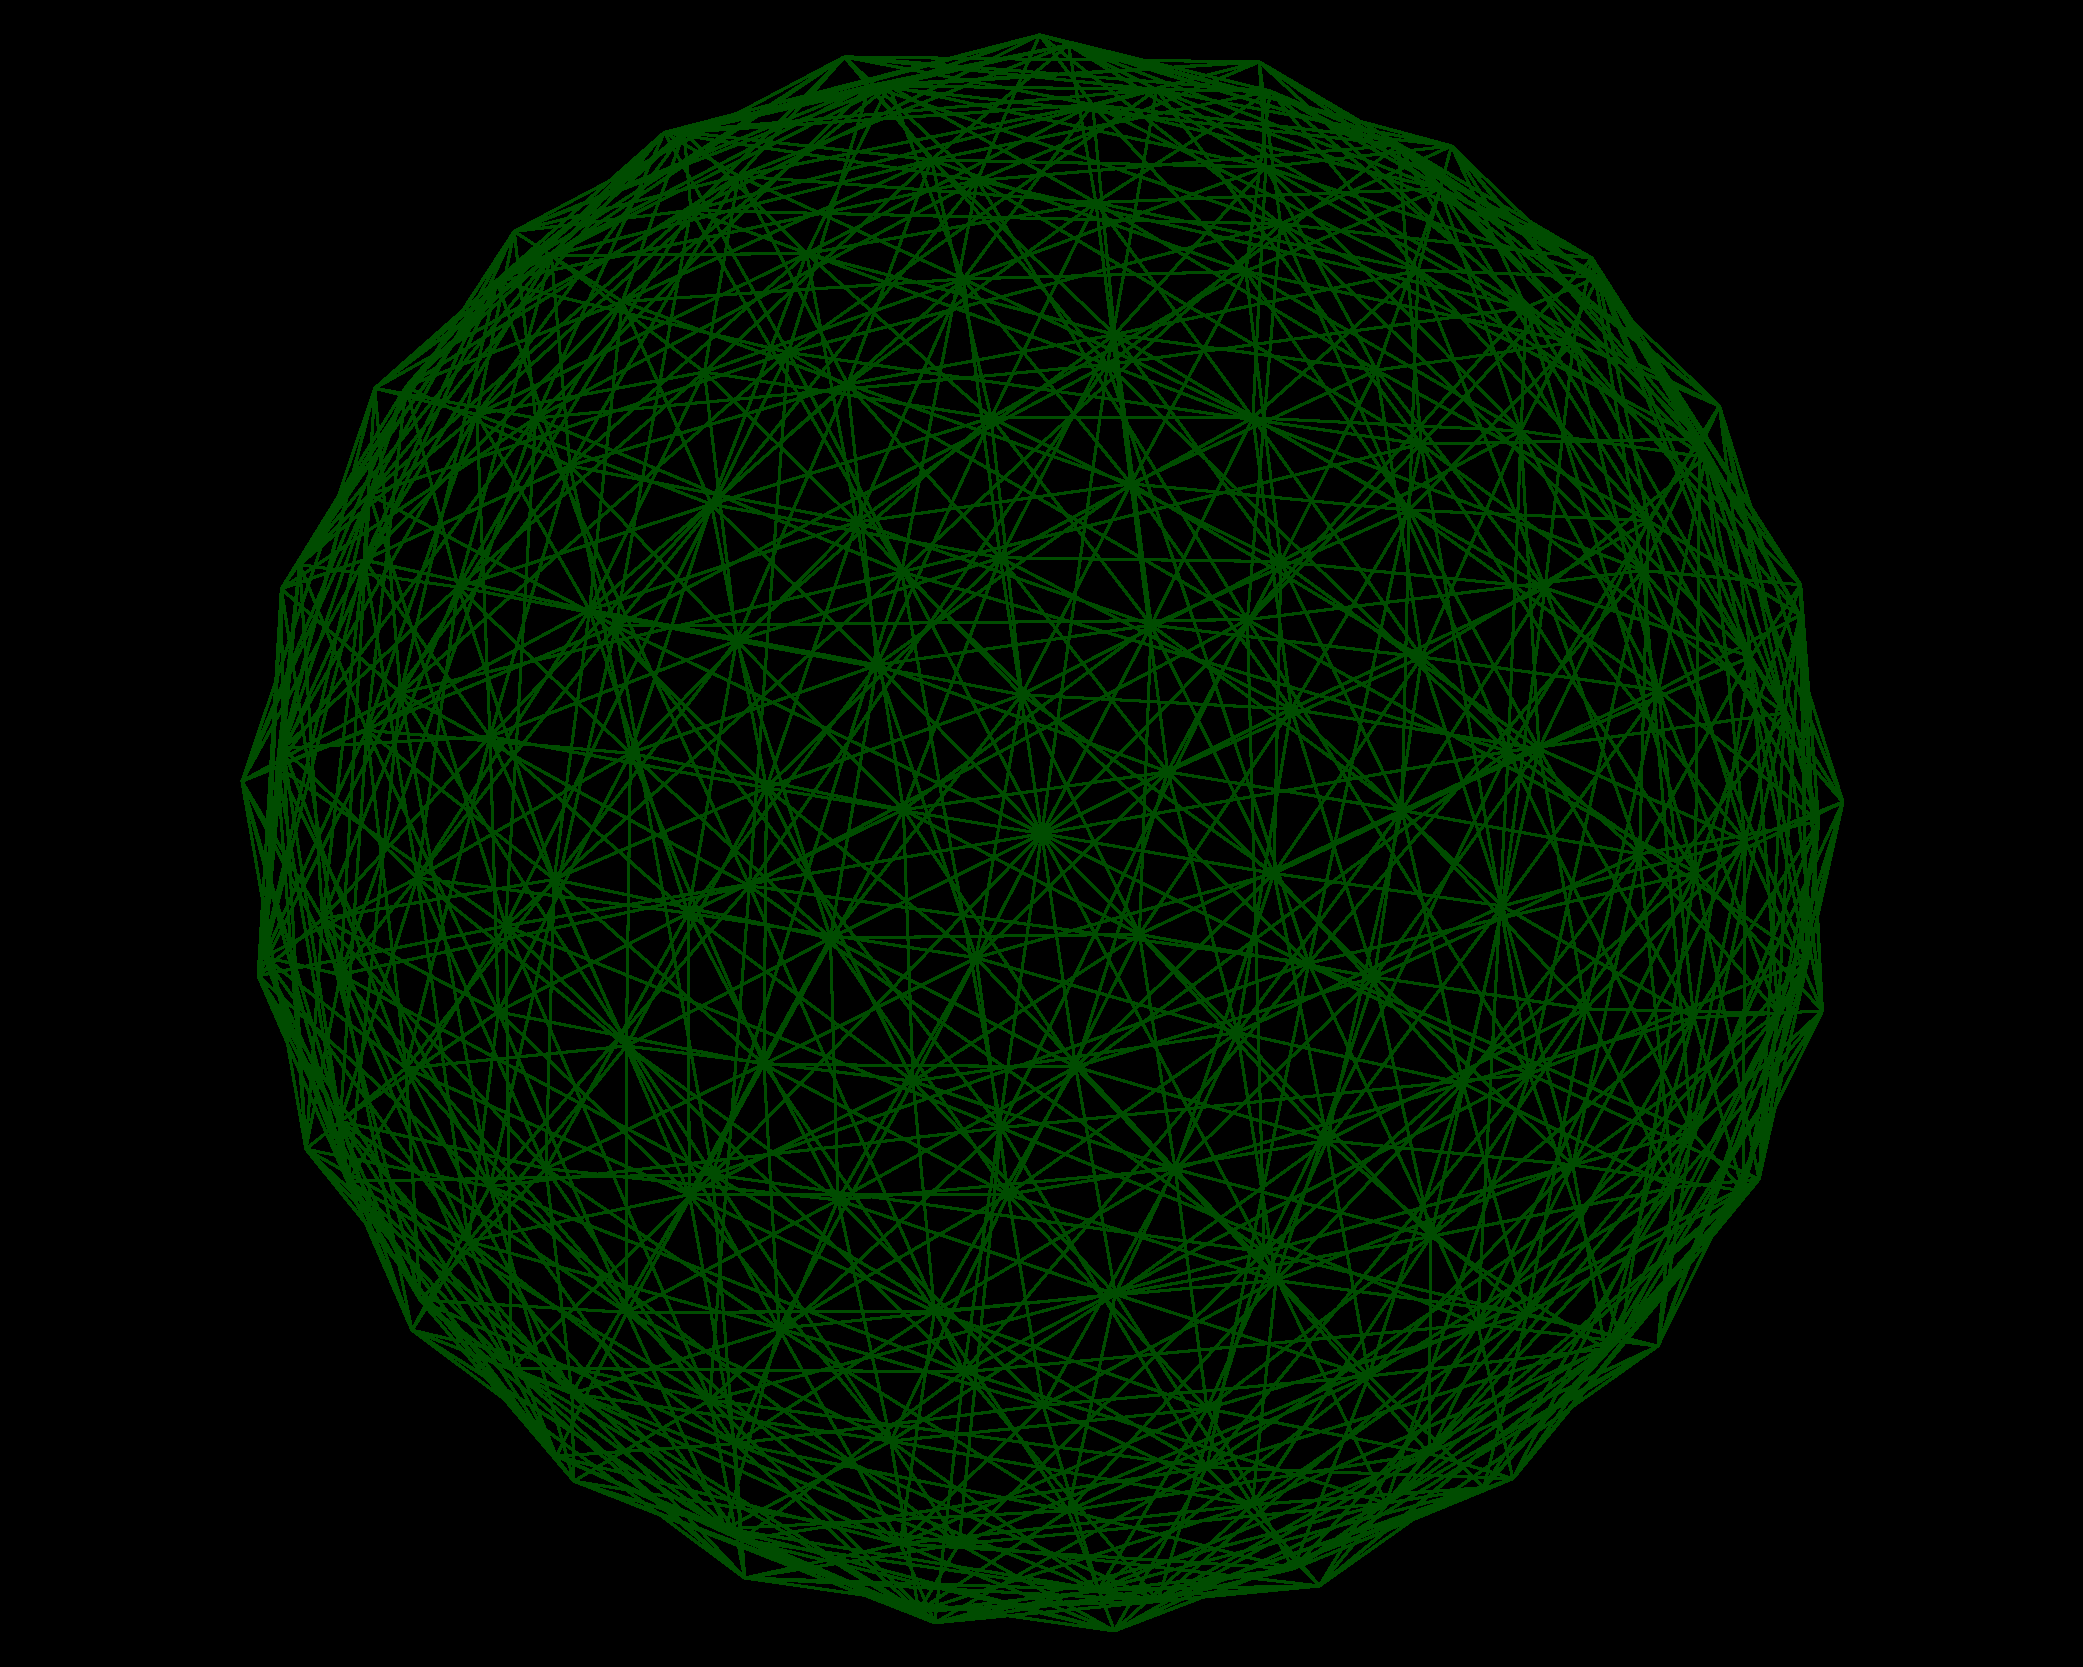
\includegraphics[width=0.4\paperwidth]{chapters/chapter3/program_viz4.pdf}}
\end{minipage}\hfill
\begin{minipage}[b]{0.5\linewidth}
\center{\includegraphics[width=0.4\paperwidth]{chapters/chapter3/program_viz3.pdf}}
\end{minipage}\hfill
\begin{minipage}[b]{0.5\linewidth}
\center{\includegraphics[width=0.4\paperwidth]{chapters/chapter3/program_viz2.pdf}}
\end{minipage}\hfill
\begin{minipage}[b]{0.5\linewidth}
\center{\includegraphics[width=0.4\paperwidth]{chapters/chapter3/program_viz1.pdf}}
\end{minipage}\hfill
\caption{Пример визуализации раскраски.}
\label{chapter3:fig:viz}
\end{figure}

\begin{statement}
\begin{equation}
\begin{split}
\chi(T^{2}(2,2)) = 8; \\
\chi(T^{2}(2,3)) = 8; \\
\chi(T^{2}(2,4)) = 8; \\
\chi(T^{2}(2,5)) = 8; \\
\end{split}
\quad\quad
\begin{split}
\chi(T^{2}(3,4)) = 8; \\
\chi(T^{2}(4,4)) = 8; \\
\chi(T^{2}(5,5)) = 8. \\
\end{split}
\end{equation}
\end{statement}

\begin{hypothesis}
Квадраты двойственных графов регулярных $(p,q)$-решений задачи Томсона (обладающих икосаэдральной симметрией) 
являются $8$-хроматическими при $p \ge 2, q \ge 2$.
\end{hypothesis}

\vspace{5pt}
\textbf{3.2 Теоретические оценки}\label{chapters:3.2}
\vspace{5pt}

В этом разделе приводятся некоторые теоретические рассуждения, продолжающие построения из первой главы. 
Как и раньше, будем обозначать как $G$ двойственный граф триангуляции для некоторой сферической диаграммы Вороного, 
удовлетворяющей условиям \ref{chapter1:eq:diams}, \ref{chapter1:eq:radiuseq}, $G^2$ -- его квадрат. 
Граф триангуляции для диаграмм Вороного с икосаэдральной симметрией обозначается $T(p,q)$.

\begin{lemma}\label{chapter3:lemma}
Пусть $G$ содержит такую вершину $v$ степени $5$, что каждая из смежных с ней вершин имеет степень $6$. 
Тогда $\chi(G^2) \ge 8$. В частности, при $p,q \ge 1$ выполнено $\chi(T^2) \ge 8$.
\end{lemma}

\begin{figure}[h]
\centering
\captionsetup{justification=centering}
\center{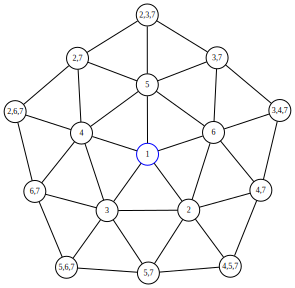
\includegraphics[width=0.45\paperwidth]{chapters/chapter3/cap.pdf}}
\caption{К лемме \ref{chapter3:lemma}.}
\label{chapter3:fig:lemma}
\end{figure}

\begin{proof}
На \figurename{ \ref{chapter3:fig:lemma}} приведены возможные цвета вершин в окрестности вершины степени $5$ (без ограничения общности). 
Тогда из вершин \enquote{внешнего} пояса не более трех имеют цвет $7$, а остальные $7$ вершин раскрашены в цвета $2$--$6$. Но это невозможно, поскольку из этих $7$ вершин можно покрасить в любой из цветов $2$--$6$ не более одной. 
\end{proof}

В заключение приведем набросок доказательства основной теоремы, 
строгая формулировка которого не была завершена в срок и будет опубликована отдельной статьей.

\begin{theorem}
При некотором $r>r_0$ для раскраски областей сферической диаграммы Вороного,
удовлетворяющей условиям \ref{chapter1:eq:diams}, \ref{chapter1:eq:radiuseq}, 
потребуется по крайней мере $8$ цветов.
\end{theorem}

\begin{myproof}[Идея доказательства.]
0. Предположим, что существует раскраска в $7$ цветов. Тогда нет области с $7$ или более сторонами (для раскраски ее $1$-окрестности потребуется $8$ цветов).

1. Тогда из леммы \ref{chapter3:lemma} следует, что не может быть $5$-угольника, окруженного $6$-угольниками. Верно ли это для вершин двойственного графа степени $3$ и $4$? В любом случае, их не может окружать полоса из $6$-угольников ширины $4$.

2. Рассмотрим подграфы, образованные вершинами степени меньше $6$. Если общий дефект компоненты связности меньше $6$, то вокруг этой компоненты раскраску $6$-угольного замощения невозможно \enquote{склеить} с собой (это возможно только в том случае, если получится цилиндр).

3. Если общий дефект равен $6$, то оценивается максимальный радиус сферы, при которым это возможно (через длину \enquote{пояса} из $6$-угольников).
\end{myproof}